\chapter{Composition des vitesses, cônes de lumière et quadrivecteurs}

\section{Deux référentiels sur une même voie ferrée}

La transformation de Lorentz établie précédemment concernait une géométrie délibérément restreinte : tous les mouvements relatifs se faisaient le long d’un seul axe. Imaginons une longue voie ferrée. Un groupe d’observateurs reste à la gare ; un autre voyage dans un train qui se déplace le long de la voie. Les directions transversales existent, mais elles n’interviennent pas tant qu’on ne les réintroduit pas plus loin.

Chaque référentiel est un système de coordonnées défini opérationnellement. Des règles graduées au repos dans le référentiel définissent les coordonnées spatiales, et des horloges synchronisées au repos dans ce référentiel définissent le temps. Le postulat qui fixe la relation entre eux est que tous les observateurs inertiels mesurent la même vitesse de la lumière.

La plupart des calculs utiliseront \(c=1\). Le temps peut être mesuré en secondes et les distances en secondes-lumière, ou en années et en années-lumière. Les vitesses sont alors des fractions sans dimension de la vitesse de la lumière. Quand on a besoin des unités usuelles, les facteurs de \(c\) sont rétablis de façon univoque par cohérence dimensionnelle ; par exemple, \(v^2\) dans un facteur de Lorentz sans dimension devient \(v^2/c^2\).

\subsection{Transformations directe et inverse}

Supposons qu’un éclair se produise quelque part dans le train ou à proximité. Il s’agit d’un seul événement, quel que soit celui qui le décrit. L’observateur à la gare lui attribue \((x,t)\), tandis que l’observateur dans le train lui attribue \((x',t')\). Dans les unités \(c=1\),
\begin{align}
x'&=\gamma_v(x-vt),&
t'&=\gamma_v(t-vx),
\label{eq:sr2-direct}\\
\gamma_v&=\frac{1}{\sqrt{1-v^2}}.
\end{align}
Newton reconnaîtrait le déplacement \(x-vt\) ; le facteur \(\gamma_v\) et le mélange de \(x\) dans \(t'\) sont les modifications relativistes.

\begin{figure}[htbp]
\centering
\includegraphics[width=0.90\textwidth]{lecture_02_figure_01.png}
\caption{Transformation de Lorentz directe reliant les coordonnées de la gare \((x,t)\) aux coordonnées du train \((x',t')\).}
\lectureframe{00:07:52}
\end{figure}

La réciprocité donne la transformation inverse en changeant le signe de la vitesse relative :
\begin{align}
x&=\gamma_v(x'+vt'),&
t&=\gamma_v(t'+vx').
\label{eq:sr2-inverse}
\end{align}
La gare n’est pas au repos de façon absolue. C’est simplement le référentiel désigné par les coordonnées non primées, et le train la voit se déplacer à \(-v\).

\begin{figure}[htbp]
\centering
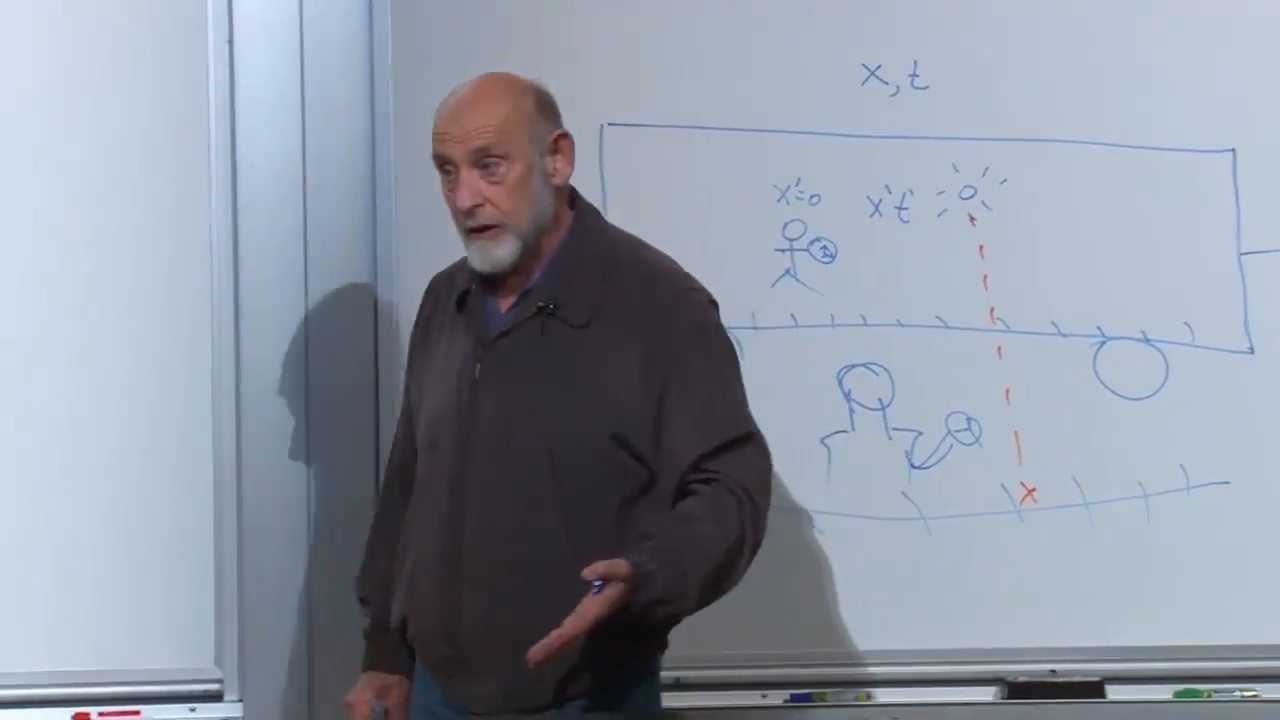
\includegraphics[width=0.90\textwidth]{lecture_02_figure_02.png}
\caption{La transformation inverse a le même facteur de Lorentz et le signe opposé pour la vitesse relative.}
\lectureframe{00:09:15}
\end{figure}

Pour un boost le long de \(x\), les coordonnées transversales ne changent pas :
\begin{equation}
y'=y,
\qquad
z'=z.
\end{equation}

On peut déterminer la vitesse relative à partir de l’équation spatiale sans examiner son dénominateur. L’origine du train est définie par \(x'=0\), et donc
\begin{equation}
x'=0
\quad\Longleftrightarrow\quad
x-vt=0
\quad\Longleftrightarrow\quad
x=vt.
\label{eq:sr2-origin-worldline}
\end{equation}
Le coefficient de \(t\) dans cette ligne d’univers est la vitesse du train dans les coordonnées de la gare.

\section{Trois référentiels et composition des boosts}

Plaçons une petite voiturette dans le train. Le train se déplace à la vitesse \(v\) par rapport à la gare, tandis que la voiturette avance dans l’allée à la vitesse \(u\) par rapport au passager du train. Désignons par \(w\) la vitesse de la voiturette par rapport à la gare. L’intuition newtonienne suggère \(w=u+v\), mais il faut laisser les transformations de Lorentz trancher.

Il y a maintenant trois systèmes de coordonnées :
\begin{equation}
(x,t),\qquad (x',t'),\qquad (x'',t'').
\end{equation}
Le premier est celui de la gare, le deuxième celui du train et le troisième celui de la voiturette. Entre le train et la voiturette,
\begin{align}
x''&=\gamma_u(x'-ut'),&
t''&=\gamma_u(t'-ux'),
\label{eq:sr2-second-boost}\\
\gamma_u&=\frac{1}{\sqrt{1-u^2}}.
\end{align}

\begin{figure}[htbp]
\centering
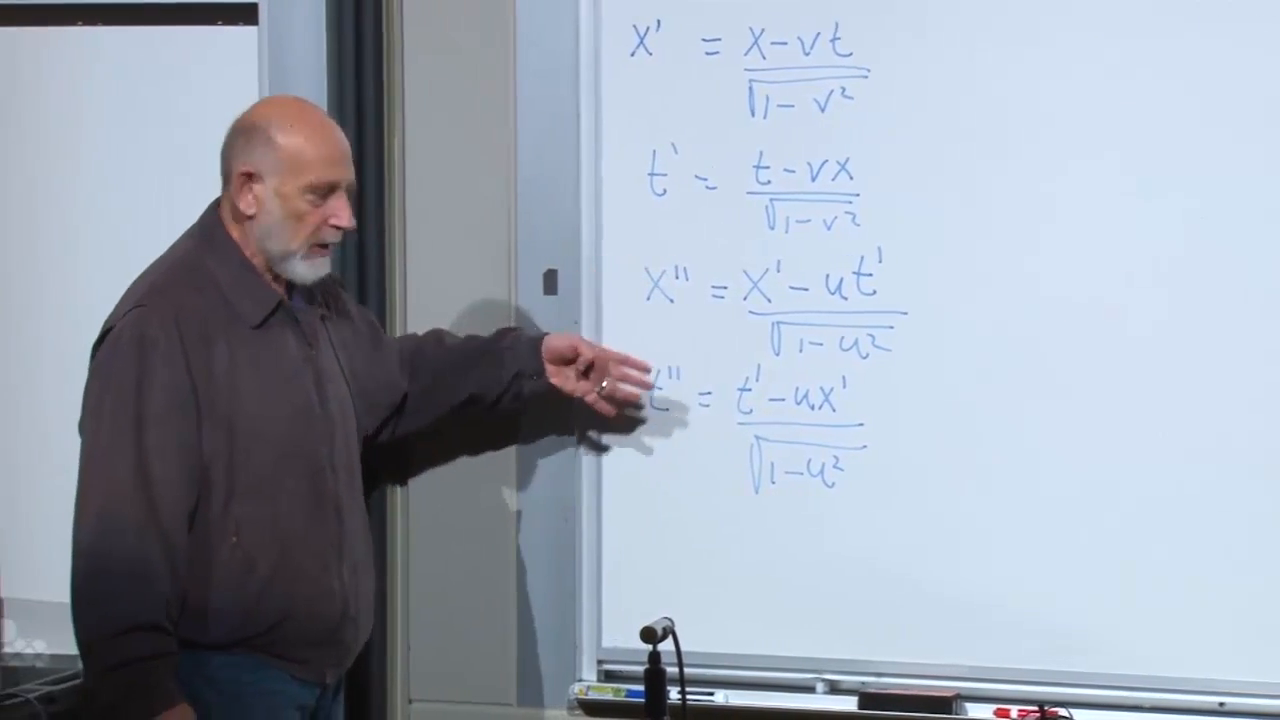
\includegraphics[width=0.90\textwidth]{lecture_02_figure_03.png}
\caption{Les formules directes de la gare au train sont suivies d’une seconde transformation de Lorentz, des coordonnées primées aux coordonnées doublement primées.}
\lectureframe{00:14:55}
\end{figure}

\subsection{Composer les boosts par substitution}

L’équation spatiale suffit pour déterminer \(w\). Substituons \eqref{eq:sr2-direct} dans la première équation de \eqref{eq:sr2-second-boost} :
\begin{align}
x''
&=\gamma_u(x'-ut')\\
&=\gamma_u\gamma_v\left[(x-vt)-u(t-vx)\right]\\
&=\gamma_u\gamma_v\left[(1+uv)x-(u+v)t\right].
\label{eq:sr2-composed-space}
\end{align}
Dans le terme \(uvx\), les deux signes moins donnent un signe plus ; les deux termes en temps se combinent en \(-(u+v)t\).

\begin{figure}[htbp]
\centering
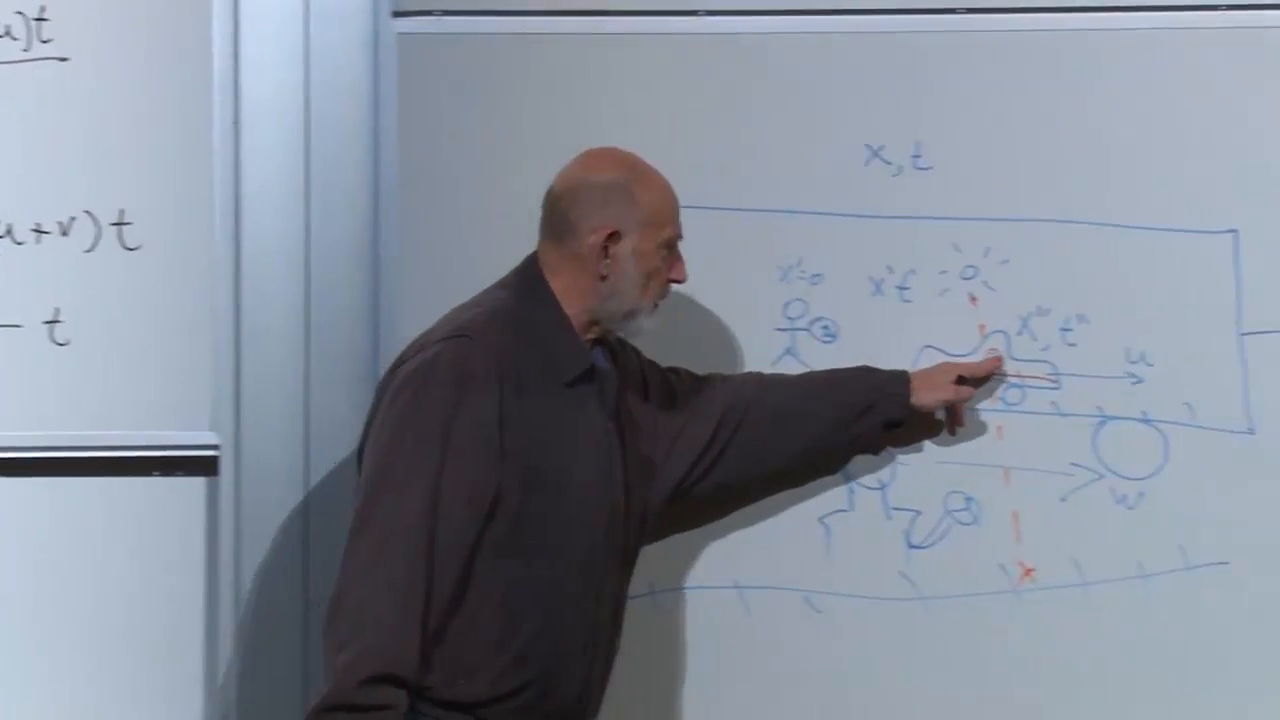
\includegraphics[width=0.91\textwidth]{lecture_02_figure_04.png}
\caption{La substitution imbriquée avant le regroupement des termes en \(x\) et en \(t\) dans le boost composé.}
\lectureframe{00:16:30}
\end{figure}

Comme précédemment, le dénominateur n’intervient pas pour repérer l’origine en mouvement. La voiturette est au repos en \(x''=0\) ; le terme entre crochets dans \eqref{eq:sr2-composed-space} doit donc s’annuler :
\begin{equation}
(1+uv)x-(u+v)t=0.
\end{equation}
Sa ligne d’univers dans le référentiel de la gare est donc
\begin{equation}
x=\frac{u+v}{1+uv}\,t,
\end{equation}
et sa vitesse est
\begin{equation}
\boxed{w=\frac{u+v}{1+uv}}.
\label{eq:sr2-velocity-add-c1}
\end{equation}

\begin{figure}[htbp]
\centering
\includegraphics[width=0.91\textwidth]{lecture_02_figure_05.png}
\caption{Le numérateur regroupé et la ligne d’univers \(x=[(u+v)/(1+uv)]t\) font apparaître la vitesse composée.}
\lectureframe{00:19:30}
\end{figure}

L’équation temporelle se compose elle aussi de façon cohérente. La transformation complète de la gare à la voiturette a la forme lorentzienne
\begin{align}
x''&=\gamma_w(x-wt),&
t''&=\gamma_w(t-wx),
\end{align}
où
\begin{equation}
\gamma_w=\frac{1}{\sqrt{1-w^2}}.
\end{equation}
En effet,
\begin{equation}
\gamma_w=\gamma_u\gamma_v(1+uv),
\end{equation}
ce qui découle de la substitution de \eqref{eq:sr2-velocity-add-c1}, suivie d’une simplification. Deux boosts colinéaires se composent donc en un autre boost colinéaire.

\subsection{Rétablir les dimensions}

\begin{classroomqa}
\audiencequestion{Pourquoi le dénominateur \(1+uv\) est-il incorrect du point de vue dimensionnel avec les unités usuelles ?}
\lecturerresponse{Il n’est correct que parce que \(c=1\) rend chaque vitesse égale à une fraction sans dimension de la vitesse de la lumière. Dans les unités usuelles, le produit doit s’écrire \(uv/c^2\), qui est sans dimension. \lecturetimestamp{00:21:11}}
\end{classroomqa}

La loi d’addition des vitesses avec les dimensions explicites est
\begin{equation}
\boxed{
w=\frac{u+v}{1+\dfrac{uv}{c^2}}
}.
\label{eq:sr2-velocity-add}
\end{equation}

\begin{figure}[htbp]
\centering
\includegraphics[width=0.90\textwidth]{lecture_02_figure_06.png}
\caption{La cohérence dimensionnelle rétablit \(c^2\) sous le produit \(uv\).}
\lectureframe{00:22:06}
\end{figure}

Pour \(\lvert u\rvert,\lvert v\rvert\ll c\),
\begin{equation}
\frac{uv}{c^2}\ll 1,
\end{equation}
et donc
\begin{equation}
w\approx u+v.
\end{equation}
L’addition newtonienne est une approximation valable aux faibles vitesses, et non une règle distincte.

\subsection{Deux régimes numériques}

Considérons d’abord
\begin{equation}
u=v=0.01c.
\end{equation}
Dans les unités \(c=1\),
\begin{equation}
w=\frac{0.02}{1.0001}\approx 0.019998.
\end{equation}
Un pour cent de la vitesse de la lumière représente déjà environ \(3\times10^6\ {\rm m/s}\), et pourtant la correction relativiste n’est que d’une part sur dix mille. Le résultat est légèrement inférieur à \(0.02c\), la valeur newtonienne.

\begin{figure}[htbp]
\centering
\includegraphics[width=0.90\textwidth]{lecture_02_figure_07.png}
\caption{Pour \(u=v=0.01c\), le dénominateur ne diffère de un que de \(10^{-4}\).}
\lectureframe{00:24:23}
\end{figure}

Considérons maintenant
\begin{equation}
u=v=0.9c.
\end{equation}
Newton prédirait \(1.8c\). La relativité donne
\begin{equation}
\frac{w}{c}
=\frac{0.9+0.9}{1+0.9^2}
=\frac{1.8}{1.81}
\approx 0.9945.
\label{eq:sr2-fast-example}
\end{equation}

\begin{figure}[htbp]
\centering
\includegraphics[width=0.90\textwidth]{lecture_02_figure_08.png}
\caption{Deux vitesses de \(0.9c\) se composent en \(1.8/1.81\), ce qui reste inférieur à la vitesse de la lumière.}
\lectureframe{00:25:48}
\end{figure}

Des boosts successifs subluminiques ne peuvent pas dépasser \(c\). Si \(u<c\) et \(v<c\), alors
\begin{equation}
1-\frac{w}{c}
=
\frac{\left(1-\frac{u}{c}\right)
      \left(1-\frac{v}{c}\right)}
     {1+\frac{uv}{c^2}}
>0.
\end{equation}
Chaque boost supplémentaire peut rapprocher le résultat de \(c\), mais jamais le faire dépasser cette valeur. À la limite \(u=c\),
\begin{equation}
w=\frac{c+v}{1+v/c}=c.
\end{equation}
La vitesse de la lumière est un point fixe de la loi de composition.

\section{La mesure des coordonnées n’est pas l’apparence visuelle}

\begin{classroomqa}
\audiencequestion{Si le train a des parois vitrées, l’observateur à la gare pourrait-il simplement regarder le passager et la voiturette ensemble et déduire directement leurs mouvements ?}
\lecturerresponse{La transformation de Lorentz concerne les mesures de coordonnées effectuées à l’aide de règles réparties dans l’espace et d’horloges synchronisées. Une image visuelle comprend aussi les temps de parcours inégaux de la lumière entre les différents événements et l’observateur. Les vitres modifient ce que l’on voit, pas la relation entre les coordonnées ; traiter une image comme un ensemble de données simultanées réintroduirait précisément l’hypothèse de simultanéité que la relativité a corrigée. \lecturetimestamp{00:27:53}}
\end{classroomqa}

Un événement a une position et une date dans chaque référentiel, que quelqu’un l’aperçoive ou non à cet instant. L’apparence optique est un sujet légitime, mais elle exige un second calcul, qui suit la lumière de chaque événement jusqu’à l’œil. Les lois de transformation sont, elles, universelles et indépendantes des parois du train.

\section{L’intervalle propre en trois dimensions spatiales}

Revenons à deux événements, l’un initialement à l’origine et l’autre en \((x,t)\). En une dimension spatiale,
\begin{equation}
\tau^2=t^2-x^2
\label{eq:sr2-interval-1d}
\end{equation}
dans les unités \(c=1\). Tous les référentiels inertiels s’accordent :
\begin{equation}
\tau^2
=t^2-x^2
=t'^2-x'^2
=t''^2-x''^2.
\end{equation}
Les coordonnées changent ; l’intervalle propre, lui, ne change pas.

Pour une séparation de genre temps, une horloge peut se déplacer d’un événement à l’autre. Si elle indique midi au premier événement, le temps écoulé qu’elle indique au second est le temps propre \(\tau\). Cette affirmation ne dépend pas du référentiel de coordonnées utilisé pour calculer l’intervalle.

\begin{figure}[htbp]
\centering
\includegraphics[width=0.90\textwidth]{lecture_02_figure_09.png}
\caption{La relation invariante entre temps propre et intervalle \(\tau^2=t^2-x^2\) est rappelée avant de réintroduire les directions transversales.}
\lectureframe{00:30:18}
\end{figure}

\subsection{Les rotations spatiales réintroduisent les directions transversales}

Considérons une rotation ordinaire des axes spatiaux avant de revenir aux boosts. Un point qui ne se trouve pas sur l’axe \(x\) a pour distance spatiale au carré
\begin{equation}
r^2=x^2+y^2+z^2,
\end{equation}
Cette quantité est invariante par rotation en vertu du théorème de Pythagore usuel. L’intervalle d’espace-temps \(3+1\) est donc
\begin{equation}
\boxed{
\tau^2=t^2-x^2-y^2-z^2
}.
\label{eq:sr2-interval-3d}
\end{equation}
Une fois \(c\) rétabli,
\begin{equation}
c^2\tau^2
=c^2t^2-x^2-y^2-z^2.
\end{equation}

\begin{figure}[htbp]
\centering
\includegraphics[width=0.90\textwidth]{lecture_02_figure_10.png}
\caption{La distance spatiale de Pythagore étend l’invariant de \(t^2-x^2\) à \(t^2-x^2-y^2-z^2\).}
\lectureframe{00:34:23}
\end{figure}

Toute combinaison de rotations spatiales et de boosts de Lorentz conserve \eqref{eq:sr2-interval-3d}. Les axes de coordonnées ordinaires attribuent des composantes différentes, mais s’accordent sur la distance euclidienne ; les référentiels inertiels d’espace-temps attribuent des composantes différentes à l’espace et au temps, mais s’accordent sur cette différence de carrés. Cet invariant est le fait géométrique central de la relativité restreinte.

\begin{classroomqa}
\audiencequestion{Si le passager remplace la voiturette par une lampe de poche dirigée vers l’avant, les observateurs du train et de la gare mesurent-ils la même vitesse de la lumière ?}
\lecturerresponse{Posons \(u=c\) dans \eqref{eq:sr2-velocity-add}. On obtient alors \(w=(c+v)/(1+v/c)=c\). Dans les unités \(c=1\), le rapport se réduit à \((1+v)/(1+v)=1\). Les deux référentiels mesurent la même vitesse, exactement comme il se doit. \lecturetimestamp{00:35:53}}
\end{classroomqa}

La question soulevée plus tôt par les parois vitrées ne remet donc pas en cause l’invariance de la vitesse de la lumière. Elle confond une mesure de coordonnées avec une image visuelle différée, et revient finalement à une confusion sur la simultanéité.

\section{Rayons nuls et cône de lumière}

En une dimension spatiale, les rayons lumineux se propageant vers la droite ou vers la gauche vérifient
\begin{equation}
x=\pm t.
\end{equation}
Leur intervalle est nul :
\begin{equation}
t^2-x^2=0.
\end{equation}
Contrairement à la distance euclidienne, un intervalle d’espace-temps nul n’exige pas que les événements coïncident. Il signifie qu’un signal lumineux peut les relier.

Lorsque toutes les directions spatiales sont réintroduites, un rayon lumineux vérifie
\begin{equation}
t^2-x^2-y^2-z^2=0,
\label{eq:sr2-null}
\end{equation}
ou
\begin{equation}
r=t
\end{equation}
pour la lumière se propageant vers le futur dans les unités \(c=1\).

\begin{figure}[htbp]
\centering
\includegraphics[width=0.90\textwidth]{lecture_02_figure_11.png}
\caption{La lumière, quelle que soit sa direction spatiale, suit une trajectoire nulle vérifiant \(t^2-(x^2+y^2+z^2)=0\).}
\lectureframe{00:39:28}
\end{figure}

En \(1+1\) dimensions, l’ensemble des trajectoires nulles est formé de deux droites \(45^\circ\). Avec deux dimensions spatiales et le temps, il prend la forme d’un cône ; trois dimensions spatiales ne peuvent pas être représentées entièrement au tableau, mais l’équation qui le définit reste inchangée.

Le cône de lumière futur est constitué des événements que la lumière émise à l’origine peut atteindre. Le cône de lumière passé est constitué des événements d’où la lumière peut atteindre l’origine. L’un s’obtient en retournant l’autre dans le temps.

\begin{figure}[htbp]
\centering
\includegraphics[width=0.90\textwidth]{lecture_02_figure_12.png}
\caption{Les rayons nuls à \(45^\circ\) engendrent les cônes de lumière futur et passé dans un diagramme d’espace-temps de dimension supérieure.}
\lectureframe{00:40:47}
\end{figure}

\begin{classroomqa}
\audiencequestion{Quel est l’invariant correspondant sous les transformations galiléennes en mécanique newtonienne ?}
\lecturerresponse{L’intervalle de temps lui-même. Tous les observateurs newtoniens s’accordent sur \(\Delta t\), même s’ils ne s’accordent pas sur le déplacement spatial. La relativité abandonne le temps universel et le remplace par l’intervalle d’espace-temps invariant. \lecturetimestamp{00:41:53}}
\end{classroomqa}

\section{Des vecteurs spatiaux aux quadrivecteurs}

Les vecteurs dont il est question ici sont des vecteurs géométriques, pas des vecteurs d’état quantiques. Un déplacement entre deux points de l’espace ordinaire a une norme et une direction. On peut translater son origine jusqu’à l’origine des coordonnées sans modifier le vecteur, et ses trois composantes peuvent se noter
\begin{equation}
x^i=(x^1,x^2,x^3)=(x,y,z),
\qquad i=1,2,3.
\end{equation}
L’indice latin \(i\) ne parcourt que les directions spatiales.

Un événement requiert une composante supplémentaire : le temps. Une position dans l’espace-temps s’écrit donc
\begin{equation}
x^\mu=(x^0,x^1,x^2,x^3)=(t,x,y,z),
\qquad \mu=0,1,2,3.
\label{eq:sr2-four-position}
\end{equation}
Par convention historique, le temps est la composante d’indice zéro, et non la quatrième :
\begin{equation}
x^0=t,\qquad x^1=x,\qquad x^2=y,\qquad x^3=z.
\end{equation}
Les indices grecs tels que \(\mu\) parcourent l’espace-temps ; les indices latins tels que \(i\) parcourent l’espace.

\begin{figure}[htbp]
\centering
\includegraphics[width=0.90\textwidth]{lecture_02_figure_13.png}
\caption{Les composantes spatiales \(x^i\) sont complétées pour former la position d’espace-temps à quatre composantes \(x^\mu=(x^0,x^1,x^2,x^3)\).}
\lectureframe{00:46:05}
\end{figure}

L’invariant devient
\begin{equation}
\tau^2
=(x^0)^2-(x^1)^2-(x^2)^2-(x^3)^2.
\end{equation}
La notation, à elle seule, n’ajoute aucune nouvelle physique. Elle permet de voir qu’une transformation de Lorentz agit linéairement sur les quatre composantes, tout comme une rotation agit linéairement sur un vecteur spatial.

\begin{classroomqa}
\audiencequestion{Puisque la transformation est linéaire, peut-on la représenter par une matrice agissant sur un vecteur colonne ?}
\lecturerresponse{Oui. Pour un boost le long de \(x\), le bloc non trivial est \(\gamma_v\begin{pmatrix}1&-v\\-v&1\end{pmatrix}\), qui agit sur \((t,x)^{\mathsf T}\), tandis que \(y\) et \(z\) restent inchangés. La notation matricielle est la manière naturelle de composer et d’organiser les transformations de Lorentz. \lecturetimestamp{00:48:14}}
\end{classroomqa}

Explicitement,
\begin{equation}
\begin{pmatrix}
t'\\x'\\y'\\z'
\end{pmatrix}
=
\begin{pmatrix}
\gamma_v&-\gamma_v v&0&0\\
-\gamma_v v&\gamma_v&0&0\\
0&0&1&0\\
0&0&0&1
\end{pmatrix}
\begin{pmatrix}
t\\x\\y\\z
\end{pmatrix}.
\label{eq:sr2-boost-matrix}
\end{equation}

\section{Déplacements et quadrivitesse}

Passons de la position d’un événement à un court segment de la ligne d’univers d’une particule. Le quadridéplacement est
\begin{equation}
\Delta x^\mu
=(\Delta t,\Delta x,\Delta y,\Delta z).
\end{equation}
Parler d’un déplacement petit annonce le calcul différentiel : \(\Delta x^\mu\) deviendra \(dx^\mu\). Pour l’instant, la notation finie rend la géométrie transparente.

L’incrément de temps propre le long d’une ligne d’univers de genre temps vérifie
\begin{equation}
(\Delta\tau)^2
=(\Delta t)^2-(\Delta x)^2-(\Delta y)^2-(\Delta z)^2.
\label{eq:sr2-proper-increment}
\end{equation}
La vitesse ordinaire est le déplacement spatial divisé par le temps coordonné et possède trois composantes. La quadrivitesse, elle, est le quadridéplacement divisé par le temps propre invariant :
\begin{equation}
u^\mu
=\frac{\Delta x^\mu}{\Delta\tau}
\quad\longrightarrow\quad
\boxed{
u^\mu=\frac{dx^\mu}{d\tau}
}.
\label{eq:sr2-four-velocity}
\end{equation}

\begin{figure}[htbp]
\centering
\includegraphics[width=0.90\textwidth]{lecture_02_figure_14.png}
\caption{Un segment de ligne d’univers définit \(\Delta x^\mu\), son invariant \(\Delta\tau\) et la quadrivitesse \(u^\mu=\Delta x^\mu/\Delta\tau\).}
\lectureframe{00:52:42}
\end{figure}

Cet objet a quatre composantes et se transforme comme un quadrivecteur. La question suivante, que nous laissons délibérément en suspens ici, est celle de sa relation avec la vitesse ordinaire à trois composantes. La résoudre nous conduira vers la quantité de mouvement relativiste, l’énergie, l’accélération et, en définitive, vers la généralisation relativiste de \(F=ma\).